\documentclass[11pt]{article}
\usepackage{amsmath}
\usepackage{amssymb}
\usepackage{graphicx,color,slashed,braket}
\usepackage{tcolorbox}
\usepackage{color}
\usepackage{tikz}
\usetikzlibrary{calc}
\usepackage[backgroundcolor=white!95!red, linecolor=cyan, bordercolor=cyan, textsize=footnotesize]{todonotes}

\begin{document}

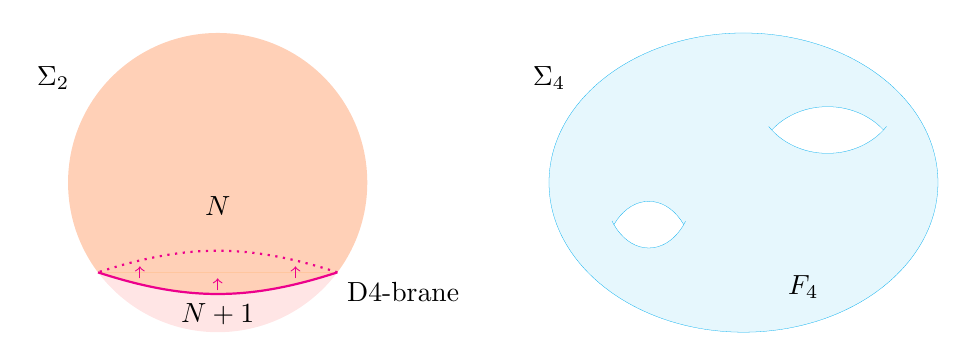
\begin{tikzpicture}[scale=0.38]
    
    \fill[color=red, opacity=0.1] (0,0) circle (5);
    \begin{scope}
        \clip (-5,-3) rectangle (5,5);
        \fill[color=orange, opacity=0.2] (0,0) circle (5);
    \end{scope}
    \fill[color=orange, opacity=0.2, even odd rule] (-4,-3) to[out=-18,in=198] (4,-3) (-4,-3) to (4,-3);
    
    \draw[thick, color=magenta, dotted] (4,-3) to[out=162,in=18] (-4,-3);
    \draw[thick, color=magenta] (-4,-3) to[out=-18,in=198] (4,-3);
    \draw[color=magenta, ->] (-2.6,-3.2) to (-2.6,-2.8);
    \draw[color=magenta, ->] (2.6,-3.2) to (2.6,-2.8);
    \draw[color=magenta, ->] (0,-3.6) to (0,-3.2);
    
    \node[] at (-5.5,3.5){$\Sigma_2$};
    \node[] at (0,-4.4){$N+1$};
    \node[] at (0,-0.8){$N$};
    \node[below right] at (4,-3){D4-brane};
    
    \begin{scope}[xshift=500pt]
        \draw[ultra thin, color=cyan, fill=white!90!cyan] (0,0) ellipse (6.5 and 5.0);
        \begin{scope}[xshift=80pt, yshift=50pt, xscale=0.8,yscale=0.6]
            \clip (0,2.2) ellipse (3 and 3.5);
            \draw[ultra thin, color=cyan, fill=white] (0,-2.2) ellipse (3 and 3.5);
        \end{scope}
        \begin{scope}[xshift=80pt, yshift=50pt, xscale=0.8,yscale=0.6]
            \clip(0,-1.8) ellipse (3 and 3.5);
            \draw[ultra thin, color=cyan] (0,2.2) ellipse (3 and 3.5);
        \end{scope}
        
        \begin{scope}[xshift=-90pt, yshift=-40pt, xscale=0.5,yscale=0.6]
            \clip (0,2.2) ellipse (3 and 3.5);
            \draw[ultra thin, color=cyan, fill=white] (0,-2.2) ellipse (3 and 3.5);
        \end{scope}
        \begin{scope}[xshift=-90pt, yshift=-40pt, xscale=0.5,yscale=0.6]
            \clip(0,-1.8) ellipse (3 and 3.5);
            \draw[ultra thin, color=cyan] (0,2.2) ellipse (3 and 3.5);
        \end{scope}
        
        \node[] at (2,-3.5){$F_4$};
        \node[] at (-6.5,3.5){$\Sigma_4$};
    \end{scope}
    
    \end{tikzpicture}

\end{document}